%**********************************************************************************
\chapter{Information distances}\label{ch:sim_structured_data}
%**********************************************************************************
%\begin{flushleft}{\slshape    
%    At the time, Nixon was normalizing relations with China.  
%    I figured that if he could normalize relations, then so could I} \\ \medskip
%    --- Edgar Codd
%\end{flushleft}
%
%SEE:\cite{Wong:1985, Lin:1991, Menendez:1997, Kullback:1951}\\
%--------------------------------------------------------------------------------------------------%
In this chapter, we explore the measurement of structural similarity in structured data.  Since increasingly more information is stored in semi-structured data formats such as XML, it makes sense not only to measure the similarity of the textual content (as in traditional information retrieval) but of its structural meta-data too. This can be very useful when, for example, extracting document types, integrating heterogeneous data sources, merging data while cleaning it, or query by example.
\section{Compression based distances}
%%%%%%%%%%%%%%%%%%%%%%%%
%\ToDo{Paraphrase All of this!}
%%%%%%%%%%%%%%%%%%%%%%%%
If Kolmogorov complexity measures the absolute information content of an object, a similarly defined measurement of information distance between two objects is the minimal information required to generate either from the other.  This measure is universal, covering all other alternative informational distances as special cases, and machine-independent.  This universality, however, prevents its computability.\cite{}

The information distance between $x$ and $y$ is the length of the shortest program to transform $x$ into $y$ and $y$ into $x$, and, up to a logarithmic additive term, is equal to the maximum of the conditional Kolmogorov complexities, which is the length of the shortest program with input $y$ that outputs $x$\cite{}.  Because it is asymmetric, the conditional complexity $K(y|x)$ alone is an unsuitable information distance, thus the algorithmic informational distance between x and y is the sum of the relative complexities, $K(y|x)+ K(x|y)$. This overestimates the information required to translate between $x$ and $y$ in case there is some redundancy between the information required to get from $x$ to $y$ and the information required to get from $y$ to $x$.

\subsection{Normalised Compression Distance}
Bennet et al. introduced an information metric between data objects in \cite{}, in which they defined information distance (ID) 
\begin{equation}
	ID(x, y) = \max \{K(x|y), K(y|x)\}
\end{equation}
and its normalized version (NID):
\begin{equation}
    NID(x, y) = \frac{\max \{K(x | y), K(y | x)\}}{\max \{K(x), K(y)\}}
\end{equation}
They also showed it to have, despite minor infringements, metric properties.  

Although, as we have discussed, Kolmogorov complexity is not computable, it can be viewed as the length of the best possible compression of $x$. The best compression, however, is also not computable, but it is approximated using standard compression algorithms. In \cite{}, Cilibrasi and Vitanyi defined a normalized compression distance (NCD), derived from NID, replacing the denominator $K(x)$ with $C(x)$, which is the length of the compressed x, and the numerator first to 
\begin{equation}
\max\{K(x, y) - K(x), K(x, y) - K(y)\}
\end{equation}
exploiting the additive property of Kolmogorov complexity \cite{}, then -- as it is easier to handle concatenation with compression -- to \begin{equation}
\min\{C(xy), C(yx)\} - \min\{C(x), C(y)\}
\end{equation} The symmetry of many compression algorithms allows a further simplification to 
\begin{equation}
C(xy) - \min\{C(x), C(y)\}
\end{equation}
arriving at the definition of NCD found in \cite{}
\begin{equation}
    NCD(x, y) = \frac{C(xy) - \min \{C(x), C(y)\}}{\max \{C(x), C(y)\}}
\end{equation}

\subsection{Crossparsing Distance}
Ziv and Merhav\cite{} showed that crossparsing two sources can be used to approximate the relative entropy (or KL-divergence) between them, in the same way that the Lempel-Ziv\cite{} showed self-parsing (compression) approximates the entropy of a single source.  In \cite{}, Helmer defined crossparsing distance (CPD) using a generalized definition of crossparsing to allow sequences of differing length. 

%\begin{myexample}{Crossparsing}
%Crossparsing a string $x$ with respect to string $y$ is defined as follows: First, find the longest prefix of $x$ that appears as a string in $y$, %i.e., find the largest integer $k$ such that $x_1, x_2, \ldots, x_k = y_i, y_{i+1}, \ldots, y_{i+k-1}$ for some $i$.  After determining the first %value for $k$, we find the longest prefix of $x$ starting with $x_{k+1}$ with respect to $y$. We continue doing so until we have parsed the whole %word $x$. The crossparsing of $x$ with respect to $y$ is the set of all resulting phrases of $x$ and is denoted with $s(x|y)$.  For example, the %crossparsing of word $x = abbbbcaabba$ with respect to word $y = baababaabba$ is the set of phrases $s(x|y) = \{abb, bb, c, aabba\}$. 
%\end{myexample}

They defined CPD by normalising and symmetrising as follows:  First, using the codebook $s(x|y)$ -- which is the multiset of phrases of $x$ resulting from the crossparsing of $x$ with respect to $y$ -- they normalize to $\frac{|s(x|y) \setminus {y}|}{|x|}$, by observing that there is at least one phrase if $x$ is found as a substring of $y$ and at most $|x|$ phrases, thus $1 \leq |s(x|y)| \leq |x|$. This gives the value 0 if $x = y$, and a maximum value of 1. Note that $s(x|y) \setminus {y}$ removes a single copy of $y$ from the multiset $s(x|y)$, even if multiple copies exist. Secondly, a symmetric distance arises by taking the mean of normalised crossparsing both ways:
\begin{equation}
CPD(x, y) = \frac{1}{2}\left(\frac{|s(x|y) \setminus {y}|}{|x|} + \frac{|s(y|x) \setminus {x}|}{|y|}\right)
\end{equation}

Helmer found CPD performed better than the NCD at clustering and classification tasks, showing the limitation of compression distance: there is only a certain window when the difference between two data objects is measured. The Gzip algorithm first builds a dictionary for $x$; the difference between $x$ and $y$ is only measured when $y$ is parsed, since at that point $y$ is encoded using a code created for $x$. As the parsing of $y$ continues, more of the encoding will rely on the parts of $y$ that has already been scanned and less from the dictionary for $x$. Puglisi et al. \cite{} interpret this as a process in which the compression algorithm learns how to encode $y$ and unlearns how to do so for $x$. CPD, however, does not display this effect, since $x$ is used to encode $y$ and vice versa, thus, avoiding the consideration of self-similarity when comparing objects.

The trouble with both CPD and NCD is that neither is a true metric.  CPD does not satisfy triangle inequality, and while NCD satisfies triangle inequality up to an additive constant, this is not very pragmatic for similarity search.
%--------------------------------------------------------------------------------------------------%
\section{Statistical distances}
%
Where Kolmogorov Complexity is the absolute information content of an object, entropy is its expected information content and a limit on its best possible compression\cite{}.  The compression distances above all rely on a string representation of the objects to compress and derive an approximate value for Kolmogorov Complexity; in the following, we consider the statistical properties of an object to derive its entropy directly. We calculate a form of structural complexity, which we use as the basis for a distance function.  Avoiding Kolmogorov complexity in this way allows a computable function that does not rely on approximation.

%The similarity of structures is quantified in terms of a relationship between their individual complexities and the complexity of a theoretical merge. 
\subsection{Structural entropic distance (SED)}
%
Recall that the Kolmogorov Complexity of a string is the size of the smallest program that generates that string.  We require structural complexity  to behave much the same way for structured objects: The joint complexity should equal the individual complexities when both structures are identical, and should equal the sum of the individual complexities when there is no common structure.  

Consider a structured object as a conceptual generator of a stream that represents all possible navigation operations.  Suppose an infinite process of random traversals gives the probability of a traversal; the collection of all traversals with associated probabilities is called an ensemble.  Let $X$ be the source emitting the stream of navigation events $E = \{ e_1, e_2, \ldots, e_n \}$ with associated probabilities $P = \{ p_1, p_2, \ldots, p_n\}$. Assuming each traversal is independent the entropy of the stream is:  
\begin{equation}
	H_b(X) = -\sum_i p_i \log_b p_i
\end{equation}
which is the average information of the events in the stream $E$.  To eliminate the dependence on the logarithmic base we define the structural complexity
\begin{equation}
	C(X) = b^{H_b(X)}
\end{equation} 

In Algorithmic information theory, joint complexity is the complexity of the concatenation of two strings\cite{}; with structured data, however, this approach would be undesirable, since concatenation does not represent a merge.  Instead we merge  the streams event by event, taking half from each.  Formally, let $X$ and $Y$ be the sources emitting the streams $E$ and $F$; let $Z$ be the notional source emitting the merged stream $G = \{g_1, g_2, \ldots, g_n\}$ where $E \subseteq G$ and $F \subseteq G$, then  
\begin{equation}
	P_Z(g_i) = \frac{P_X(g_i) + P_Y(g_i)}{2}
\end{equation}

We define structural entropic distance, notionally, as the ratio of the joint complexity to the geometric mean of individual complexities, normalised into the range $[0,1]$, which can now be defined concretely using structural complexity: 
\begin{equation}
SED(X,Y) = \frac{C(Z)}{\sqrt{C(X) \cdot C(Y)}} - 1
\end{equation}
This distance is guided by the requirements of having a distance based on the amount of overlap of structural similarity. 
\nociteown{Moss:2013,Connor:2013a,Connor:2013b,Connor:2012,Connor:2011,Connor:2011a}
\nociteothers{Moss:2013, Connor:2013a,Connor:2013b,Connor:2012,Connor:2011,Connor:2011a}
\subsection{Relationship to Jensen-Shannon divergence}
The above distance function turns out to have a great deal of commonality with the Jensen-Shannon divergence (JSD), as shown by Theorem \ref{proof:JS}, and is a semantically compelling metric; for any data type that can be characterised by an ensemble of event-probability pairs, the Jensen-Shannon similarity gives an estimate of the probability of that data's having been output by the same probabilistic generator.
\begin{mytheorem}{$SED(x,y) = b^{JSD(x,y)} - 1$}
\begin{proof}\label{proof:JS}\footnotesize
\begin{align}
SED(X,Y) &= \frac{C(Z)}{\sqrt{C(X) \cdot C(Y)}} - 1\\
%
&= \frac{b^{H_b(Z)}}{\sqrt{\strut b^{H_b(X)} \cdot b^{H_b(Y)}}} - 1\\
%
&= \frac{b^{H_b(X)}}{\strut b^{\frac{1}{2}(H_b(X) + H_b(Y))}} - 1\\
%
&= b^{H_b(Z) -\frac{1}{2}(H_b(X) + H_b(Y))} - 1
\end{align}
Consider now only the exponent:
\begin{equation}
H_b(Z) -\frac{1}{2}(H_b(X) + H_b(Y))
\end{equation}
Substituting in the definition of entropy:
\begin{equation}
-\frac{1}{2}\sum_e 2 \cdot P_{Z}(e) \log_b P_{Z}(e) - P_{X}(e) \log_b P_{X}(e) - P_{Y}(e) \log_b P_{Y}(e)
\end{equation}
and rewriting in the positive:
\begin{equation}
\frac{1}{2}\sum_e -2 \cdot P_{Z}(e) \log_b P_{Z}(e) + P_{X}(e) \log_b P_{X}(e) + P_{Y}(e) \log_b P_{Y}(e)
\end{equation}
and substituting in the definition of $P_{Z}(e)$
\begin{equation}
\frac{1}{2}\sum_e -(P_{X}(e) + P_{Y}(e)) \log_b P_{Z}(e) + P_{X}(e) \log_b P_{X}(e) + P_{Y}(e) \log_b P_{Y}(e)
\end{equation}
then simplifying
\begin{equation}
\frac{1}{2}\sum_e P_{X}(e)\cdot ( \log_b P_{X}(e) - \log_b P_{Z}(e)) + P_{Y}(e) \cdot ( \log_b P_{Y}(e) - \log_b P_{Z}(e))
\end{equation}
and combining logs gives:
\begin{equation}
\frac{1}{2}\sum_e P_{X}(e) \log_b \frac{P_{X}(e)}{P_{Z}(e)} + P_{Y}(e) \log_b \frac{P_{Y}(e)}{P_{Z}(e)}
\end{equation}
which as shown in equation \ref{eq:jsd} is the Jensen-Shannon divergence, thus,
\begin{equation}
SED(X,Y) = b^{JSD(X,Y)} - 1
\end{equation}

\end{proof}
\end{mytheorem}

In this context, the JSD is considered as an assessment of the difference of two independent probability distributions: that is, where a randomly sampled event has a number of different possible outcomes, each with its own assigned probability.

This probabilistic divergence model can be applied to many other data sets, essentially any set of data whose semantics can be usefully captured in a vector space model. For example, in Information Retrieval, the unigram generative model (see e.g. \cite{manning:book,rijsbergen:1979}) has long been successfully used as a basis of similarity estimation among documents. In this model, a document is essentially reduced to a probabilistic generator, generating the terms within the document with probabilities in ratio to the number of appearances of each. Any such probabilistic metric can then be applied over these probability distributions to give a measurement of document similarity.  We look at this further in chapter \ref{ch:ir}.  Many other contexts, for example the extraction of image features, can also be viewed as such a probabilistic generative process.
%--------------------------------------------------------------------------------------------------%
\section{Structured data}
Both compression-based and statistical distances require, for structural comparison, a representation of the structured object that excludes the content, leaving only the structural information.  With compression based distances only a string representation is required, so a traversal that outputs the structural data is sufficient.  Statistical distances, however, require a distribution of events to be constructed upon which a probabilistic model is built; this requires a series of random traversals, meanwhile keeping track of the frequency of structural events.

\subsection{String representations}
In his comparison of NCD and CPD, Helmer\cite{} used four different methods to extract structural information from XML documents
\begin{description}
\item[Tags] Strip XML documents of all content (e.g. text nodes and attribute values) and extract all other nodes in document order by outputting their tag names (both opening and closing) and possible attribute names.
\item[Pairwise] Remove all content from the XML document and keep the remaining structural nodes. For each node, however, prepend the name of the parent node to its name. Again the document order is maintained but no closing tags are output.
\item[Full Path] After removing the content, prepend node names to the full path from the root node to the current node.
\item[Family Order] Family Order traversal represents a compromise between breadth-first and depth-first traversal. All the children of a node are output en bloc. However, before doing so, all their descendants have to be processed. 
\end{description}

%One could argue that describing the structural information of an XML document in a breadth-first manner is as appropriate as traversing it in document order. However, breadth-first traversal is problematic due to its memory consumption: given an XML document of height h, breadth-first traversal may need space that is exponential in h, whereas depth-first traversal uses up space that is linear in h.  In this way we still manage to keep the sibling information intact without having to store whole levels of the tree during the traversal.
\subsection{Statistical representation}
Extracting structural information for Statistical distances require a little more treatment; using the tree as a conceptual generator of events, an event stream is output by a random walk of the tree.  These events collectively form an ensemble of event-probability pairs from which the entropy is calculated.
\begin{figure}\footnotesize
\trimbox{0mm 0mm 0mm -10mm}{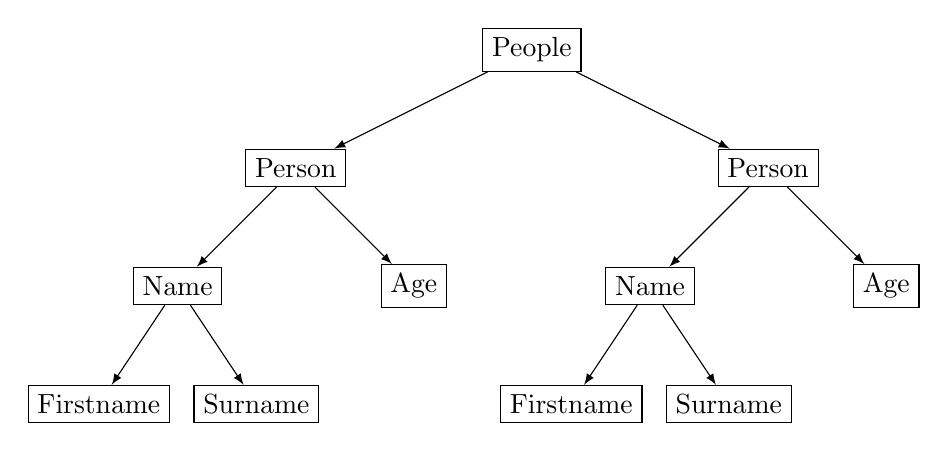
\begin{tikzpicture}[level/.style={sibling distance=60mm/#1}, edge from parent/.style={draw,-latex}]
\node [draw] (z){People}
  child {node [draw] (a) {Person}
    child {node [draw] (b) {Name}
        child {node [draw] (d) {Firstname}}
        child {node [draw] (e) {Surname}}
    }
    child {node [draw] (g) {Age}
    }
  }
  child {node [draw] (j) {Person}
    child {node [draw] (l) {Name}
      child {node [draw] (o) {Firstname}}
      child {node [draw] (p) {Surname}}
    }
    child {node [draw] (k) {Age}}
};
\end{tikzpicture}
}\\
\trimbox{0mm 0mm 0mm -10mm}{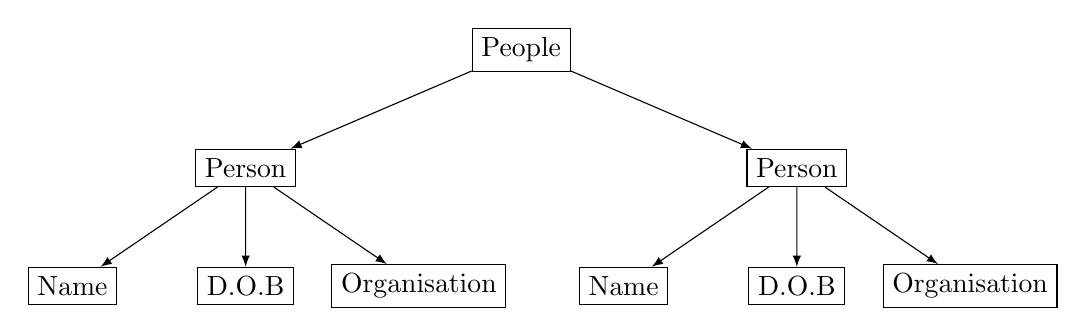
\begin{tikzpicture}[edge from parent/.style={draw,-latex}]
\tikzstyle{level 1}=[sibling distance=70mm] 
\tikzstyle{level 2}=[sibling distance=22mm] 
\node [draw] (z){People}
  child {node [draw] (a) {Person}
    child {node [draw] (c) {Name}}
    child {node [draw] (d) {D.O.B}}
    child {node [draw] (e) {Organisation}}
  }
  child {node [draw] (b) {Person}
    child {node [draw] (f) {Name}}
    child {node [draw] (g) {D.O.B}}
    child {node [draw] (h) {Organisation}}
  };

\end{tikzpicture}
}\caption{Trees used to generate an ensemble of events}
\label{ex:tree}
\end{figure}

\begin{table}\footnotesize
\centering
\begin{tabular*}{\textwidth}{l @{\extracolsep{\fill}}lrrr}
\toprule
event $e$		&$P_X(e)$\		&$P_Y(e)$		&$P_{Z}(e)$\\
\midrule
/People & $\frac{1}{33}$ & $\frac{1}{23}$ & $\frac{56}{759}$\\
/People/Person & $\frac{2}{33}$ & $\frac{2}{23}$ & $\frac{112}{759}$\\	
/People/Person/Name & $\frac{2}{33}$ & $\frac{2}{23}$ & $\frac{112}{759}$\\	
/People/Person/Age & $\frac{2}{33}$ & 0 & $\frac{1}{33}$\\
/People/Person/D.O.B & 0 & $\frac{2}{23}$ & $\frac{1}{23}$\\	
/People/Person/Organisation & 0 & $\frac{2}{23}$ & $\frac{1}{23}$\\
/People/Person/Name/Firstname & $\frac{2}{33}$ & 0 & $\frac{1}{33}$\\
/People/Person/Name/Surname & $\frac{2}{33}$ & 0 & $\frac{1}{33}$\\
/Person & $\frac{2}{33}$ & $\frac{2}{23}$ & $\frac{112}{759}$\\
/Person/Name & $\frac{2}{33}$ & $\frac{2}{23}$ & $\frac{112}{759}$\\
/Person/Age & $\frac{2}{33}$ & 0 & $\frac{1}{33}$\\
/Person/D.O.B & 0 & $\frac{2}{23}$ & $\frac{1}{23}$\\
/Person/Organisation & 0 & $\frac{2}{23}$ & $\frac{1}{23}$\\
/Person/Name/Firstname & $\frac{2}{33}$ & 0 & $\frac{1}{33}$\\
/Person/Name/Surname & $\frac{2}{33}$ & 0 & $\frac{1}{33}$\\
/Name & $\frac{2}{33}$ & $\frac{2}{23}$ & $\frac{112}{759}$\\
/Name/Firstname & $\frac{2}{33}$ & 0 & $\frac{1}{33}$\\	
/Name/Surname & $\frac{2}{33}$ & 0 & $\frac{1}{33}$\\
/Age & $\frac{2}{33}$ & 0 & $\frac{1}{33}$\\	
/Firstname & $\frac{2}{33}$ & 0 & $\frac{1}{33}$\\	
/Surname & $\frac{2}{33}$ & 0 & $\frac{1}{33}$\\	
/D.O.B & 0 & $\frac{2}{23}$ & $\frac{1}{23}$\\	
/Organisation & 0 & $\frac{2}{23}$ & $\frac{1}{23}$\\	
\bottomrule
\end{tabular*}
\caption{all of the events generated by random walks and their probabilities}
\label{event_table}
\end{table}

Consider the two trees in example \ref{ex:tree}, a stream of events is generated by a \textit{random walk} markov process over the tree structure.  A start node is selected at random, then at each step either an edge is traversed or the process is exited. Once the process is exited the resultant path forms an event in the probability space. An equivalence relation is formed on paths that contain a sequence of nodes with identical labels, that is, two different paths may be considered an instance of the same event if their sequence of node labels are identical.  We can then calculate the probabilities of the events by simply enumerating all possible paths in the tree and counting the occurrences of each event.  Table \ref{event_table} shows the probabilities of each event in both trees, along with the probabilities of the merged stream.

\subsection{Mapping the statistical reprenentation to a vector space}\label{vector_space}
Many important similarity applications make use of the vector space model, where data objects can be represented as points in a space (for more information consult chapter \ref{ch:distance}).  The compression based distances do not lend themselves to this kind of treatment, not least because they do not satisfy Triangle Inequality.  The statistical distances do, however.

Using this mapping, tree structured data can easily be adapted to existing similarity applications.  We can, furthermore, now treat trees simply as vectors in a vector space and benefit from the abstraction knowing that any mathematical treatment applies to the whole domain, and indeed any other.  We now show the mapping from a frequency table of events to a vector space, and the calculation of JSD for vectors in $\mathrm{R}^n$.

Consider an inner product space over $\mathrm{R}^n$, where each dimension $x_i$ corresponds to a count of event $e_i$.  We use the norm: 
\begin{align}
    \|\mathbf{x}\|_1 &= \sum_{i=1}^{n} |x_i|
\intertext{to produce the unit vector:}
    \hat{\mathbf{x}} &= \frac{\mathbf{x}}{\|\mathbf{x}\|_1}
\intertext{where each $\hat{x}_i$ corresponds to the probability of observing event $e_i$.  Now, let the information vector of $\mathbf{x}$ be:}
    \mathbf{i}_x &= -\log_b(\hat{\mathbf{x}})
\intertext{where each $i_j$ is the amount of information gained by observing event $e_j$.  We can use the inner product:}
\langle \mathbf{x}, \mathbf{y}\rangle &= \sum_{i=1}^n x_i y_i
\intertext{to calculate the entropy as the inner product of the unit vector $\hat{\mathbf{x}}$ and the information vector $\mathbf{i}_x$:}
    H_b(\mathbf{x}) &= \langle \hat{\mathbf{x}} , \mathbf{i}_x\rangle
\intertext{which is the total information in the vector $\mathbf{x}$.	  And finally calculate the Jensen-Shannon divergence as,} 
	JSD(\mathbf{x}, \mathbf{y}) &= H_b(\mathbf{z}) - \frac{1}{2}(H_b(\mathbf{x}) + H_b(\mathbf{y}))
\end{align}
where $\mathbf{z} = \frac{\hat{\mathbf{x}} + \hat{\mathbf{y}}}{2}$ is the centroid of the unit vectors.
\begin{figure}
  \centering
  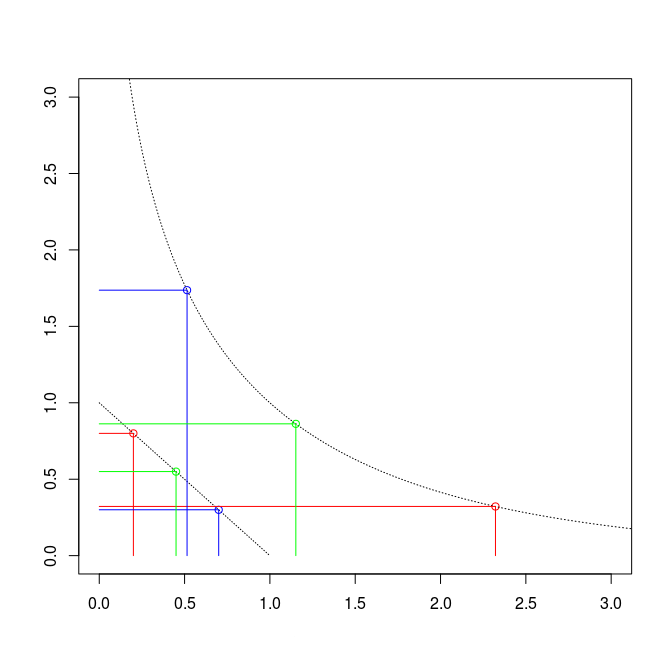
\includegraphics[width=4in]{gfx/sed_vector}
  \caption[Calculating distance]
   {In two dimensions -- The unit vectors $\hat{\mathbf{x}}$ (red), $\hat{\mathbf{y}}$ (blue), and $\hat{\mathbf{z}} = \frac{\hat{\mathbf{x}} + \hat{\mathbf{y}}}{2}$ (green) are on the $L^1$ norm; and the information vectors (using base 2), $\mathbf{i}_x$, $\mathbf{i}_y$, $\mathbf{i}_z$ are on the curved line.  The entropy is the dot product of the unit vector and information vector.  As the unit vector moves to the extremes in one direction the }
   \label{fig:entropic_space}
\end{figure}

Plotting some of these vectors in two-dimensional spaces gives us some intuition for how this function behaves.  As figure \ref{fig:entropic_space} demonstrates, the highest entropies occur when the normalised points lie at the extreme ends of the norm; by implication distances are far larger at the extremes than its Euclidean representation might suggest.  When a point has one dimension that is very low, it pushes that point much further away from other points that do not.  And this is, in fact, desirable behaviour for many similarity applications, such as clustering.  
%--------------------------------------------------------------------------------------------------%

%--------------------------------------------------------------------------------------------------%
\section{Conclusion}
This chapter has shown that existing information theoretic measures of structural distance based upon compression may not be suitable for similarity search.  We have produced an alternative, SED, that uses entropy at its core, which in turn has many commonalities with Jensen-Shannon Divergence.  

The transformation of JSD for use with metric searching prohibitively increases its dimensionality.  We have shown that SED, however, which can be used in its raw form for tree structured data, allows for much greater pruning opportunities with a metric index.  Furthermore, through algebraic manipulation, it can be calculated efficiently; by using an inverted index data structure, and, for range queries, early termination, this saving is as much as two orders of magnitude.
